\documentclass[referee,pdflatex,sn-basic]{sn-jnl}% Basic Springer
\usepackage{lmodern}
\usepackage{fix-cm}
\jyear{2026}%

\theoremstyle{thmstyleone}%
\newtheorem{theorem}{Theorem}%
\newtheorem{proposition}[theorem]{Proposition}%
\theoremstyle{thmstyletwo}%
\newtheorem{example}{Example}%
\newtheorem{remark}{Remark}%
\theoremstyle{thmstylethree}%
\newtheorem{definition}{Definition}%
\raggedbottom

\usepackage{multirow}
\usepackage{xcolor}
\usepackage[utf8]{inputenc}
\usepackage{amsmath}
\usepackage{amssymb}
\usepackage{algorithm}
\usepackage{algpseudocode}
\usepackage{array}
\usepackage{tabularx}
\usepackage{hhline}
\usepackage{balance}
\usepackage{soul}
\usepackage{stackengine}
\usepackage{graphicx}
\graphicspath{{Figures/}{./}}
\usepackage{lineno}
\usepackage{hyperref}

\linenumbers

\begin{document}

\title[Short-Term Precipitation Forecasting over Dublin]{Short-Term Regional Precipitation Forecasting over Dublin Using ERA5 Reanalysis: Robustness, Probabilistic Reliability, and Predictor Attribution}

\author[1,2]{\fnm{Yue} \sur{Li}}
\email{yue.li5@ucdconnect.ie}
\author*[1,2,3]{\fnm{Soumyabrata} \sur{Dev}}
\email{devs@tcd.ie}

\affil[1]{\orgname{The ADAPT SFI Research Centre}, \orgaddress{\city{Dublin}, \country{Ireland}}}
\affil[2]{\orgdiv{School of Computer Science}, \orgname{University College Dublin}, \orgaddress{\city{Dublin}, \country{Ireland}}}
\affil*[3]{\orgdiv{School of Computer Science and Statistics}, \orgname{Trinity College Dublin}, \orgaddress{\city{Dublin}, \country{Ireland}}}

\abstract{
Short-term precipitation forecasting over Dublin is challenging because of the strong temporal variability of rainfall and the maritime influence on regional weather conditions. Using 6-hourly European Centre for Medium-Range Weather Forecasts Reanalysis v5 (ERA5) data from 2004 to 2021, this study systematically evaluates reference forecasts, XGBoost, Transformer, deterministic bidirectional long short-term memory (BiLSTM) models, and probabilistic recurrent models for 6-hour-ahead prediction of Dublin regional mean precipitation. Model performance is assessed using repeated training with five fixed random seeds, rainfall-regime and threshold-based evaluation, probabilistic metrics, SHapley Additive exPlanations (SHAP) attribution, and feature ablation. BiLSTM-Attention achieved the lowest mean test root mean squared error (RMSE) of 0.2429~mm, closely followed by XGBoost at 0.2439~mm, while bootstrap analysis showed no clear difference between the two models for the full test set or wet conditions. Under heavy rainfall, however, XGBoost achieved lower error, and event-detection skill declined sharply as the rainfall threshold increased. The probabilistic recurrent models produced empirical 95\% coverage close to the nominal level over the full test set, but coverage deteriorated markedly for high-intensity rainfall, revealing substantial upper-tail undercoverage. SHAP analysis of BiLSTM-Attention identified total cloud cover, meridional wind, surface pressure, and minimum precipitation rate as influential predictors, while ablation experiments showed that total cloud cover provided more stable incremental predictive information than the highly correlated maximum precipitation rate. These results highlight the importance of regime-specific evaluation, repeated-run robustness analysis, and complementary interpretability methods in regional precipitation forecasting.
}

\keywords{Short-term precipitation forecasting, ERA5 reanalysis data, Model robustness, Probabilistic forecasting, Predictor attribution}

\maketitle

\section{Introduction}
\label{intro}

Accurate short-term precipitation forecasting is important for urban flood management, transportation safety, and water-resource planning, particularly in regions such as Ireland where weather conditions can change rapidly under strong maritime influence \citep{toth2000comparison}. Precipitation remains difficult to predict because of the nonlinear evolution of atmospheric processes, the intermittency of rainfall, and limitations in the spatial and temporal representation of meteorological observations \citep{magnusson2019ecmwf}. Numerical Weather Prediction systems, including the European Centre for Medium-Range Weather Forecasts (ECMWF) Integrated Forecasting System, provide physically based forecasts and commonly use ensemble approaches to represent forecast uncertainty. These systems are highly developed, but their computational requirements can limit their use in lightweight regional forecasting applications \citep{haiden2021evaluation}.

Machine-learning weather prediction has developed rapidly in recent years. Deep-learning architectures and large-scale models such as Pangu-Weather and FuXi have demonstrated that data-driven methods can learn complex atmospheric relationships and provide competitive forecasts with substantially lower inference cost than conventional numerical models \citep{bi2022pangu,chen2023fuxi}. At regional scales, recurrent neural networks and related sequence models are particularly suitable because meteorological predictors are naturally represented as time series. However, predictive accuracy alone does not provide a complete assessment of precipitation forecasting performance. Rainfall distributions are highly skewed, dry and low-rainfall observations are common, and high-intensity events occur much less frequently. A model that performs well over the full test distribution may therefore behave differently when evaluated specifically under stronger rainfall conditions.

Uncertainty estimation provides an additional perspective on forecast quality. Many machine-learning forecasting models are trained to produce a single deterministic prediction, whereas risk-sensitive applications also require information about the uncertainty associated with that estimate \citep{yang2024interpretable}. Probabilistic neural networks can address this issue by predicting parameters of a conditional distribution rather than a single rainfall value. However, satisfactory probabilistic performance over the full test set does not necessarily imply reliable uncertainty estimates for less frequent heavy-rainfall events. Evaluation of prediction-interval coverage and probabilistic scores across different rainfall regimes is therefore important when assessing the reliability of probabilistic precipitation forecasts.

Interpretability presents a related challenge. Deep neural networks can capture nonlinear temporal relationships but often provide limited information about how individual meteorological predictors contribute to their forecasts \citep{du2019techniques}. Attention mechanisms provide one way of weighting temporal representations, while post hoc attribution methods such as SHapley Additive exPlanations (SHAP) \citep{lundberg2017unified} can be used to examine predictor-level contributions. These interpretations should be distinguished from statistical association and predictive necessity. A variable may be strongly correlated with precipitation while providing limited additional information once closely related predictors are already included in the model. Combining correlation analysis, model attribution, and feature ablation can therefore provide a more complete assessment of predictor relevance.

Regional precipitation forecasting over Ireland provides a useful setting in which to examine these issues. Previous work has explored uncertainty-aware recurrent modelling for rainfall prediction in this region \citep{10906190}, while the rapidly changing Atlantic-influenced weather conditions continue to present challenges for localized forecasting. In this study, reference, machine-learning, deterministic deep-learning, and probabilistic recurrent models are evaluated for 6-hour-ahead regional mean precipitation forecasting over Dublin using ERA5 reanalysis data from 2004 to 2021. The analysis considers overall point-forecast accuracy, sensitivity to random initialization, performance across rainfall regimes, event-detection skill, probabilistic reliability, and predictor attribution. Particular attention is given to whether conclusions based on aggregate test performance remain valid for stronger precipitation events and whether different measures of predictor relevance lead to consistent interpretations.

\subsection{Main contributions}

The main contributions of this study are as follows:

\begin{itemize}
    \item A common experimental setting is used to compare reference forecasts, XGBoost, Transformer, deterministic BiLSTM models, and uncertainty-aware recurrent models for short-term regional precipitation forecasting over Dublin.

    \item Model robustness is assessed using repeated training with five fixed random seeds, together with rainfall-regime and threshold-based analyses that distinguish overall performance from forecasting skill under wet and heavier precipitation conditions.

    \item Probabilistic recurrent models are evaluated using negative log-likelihood, continuous ranked probability score, prediction-interval coverage, and interval width. Their reliability is examined separately for the full test distribution and the upper tail of the precipitation distribution.

    \item Predictor relevance is examined from complementary perspectives using training-only Spearman correlation, SHAP attribution, and leave-one-feature-out ablation, allowing marginal statistical association, model attribution, and incremental predictive contribution to be distinguished.
\end{itemize}

The remainder of this paper is organized as follows. Section~2 reviews related work on precipitation forecasting, machine-learning methods, probabilistic prediction, and model interpretability. Section~3 describes the study region, ERA5 dataset, feature selection, forecasting models, experimental setup, and diagnostic analyses. Section~4 presents the forecasting, robustness, probabilistic, and interpretability results. Section~5 discusses the main findings, their implications, and the limitations of the study. Section~6 summarizes the conclusions and directions for future work.

%Relatedwork----------------------------------
\section{Related work}

Recent advances in meteorological modeling have been supported by the increasing availability of high-resolution reanalysis datasets and the development of machine learning techniques, both of which have become important for precipitation forecasting, as demonstrated by \citet{10512739}. Reanalysis datasets provide temporally and spatially consistent climate information that supports retrospective climate studies and weather prediction applications \citep{10512483}. Among these products, the ERA5 reanalysis dataset developed by the European Centre for Medium-Range Weather Forecasts (ECMWF) under the Copernicus Climate Change Service represents a substantial improvement over its predecessors. \citet{hersbach2020era5} introduced ERA5 with hourly coverage and a spatial resolution of approximately 31~km, showing marked improvements over ERA-Interim in reproducing variability and extremes across multiple atmospheric variables. Subsequent evaluations have further clarified the reliability and limitations of ERA5. \citet{mcnicholl2021evaluating} found strong agreement between ERA5 near-surface air temperature and ground-based observations but also reported discrepancies under complex meteorological conditions. \citet{doddy2021reanalysis} compared several reanalysis products for renewable energy applications in Ireland and showed that ERA5 generally outperforms MERRA-2 and JRA-55, while still exhibiting regional biases that require consideration. For precipitation, \citet{lavers2022evaluation} demonstrated that ERA5 improves spatial and temporal consistency relative to previous datasets but systematically underestimates extreme events and shows reduced skill over mountainous and convective-dominated regions. \citet{palharini2021assessment} evaluated eleven satellite-based precipitation products across different regions of Brazil and found that no single product consistently captured extreme rainfall, with performance varying by region and event intensity. Similarly, \citet{kumar2025long} evaluated CHIRPS and GSMaP\_ISRO rainfall estimates against gauge observations over India during 2000--2022 and found that GSMaP\_ISRO agreed more closely with station measurements than CHIRPS, while both products diverged notably over complex terrain such as the Western Ghats. These studies show that precipitation products can provide useful regional information, but their performance remains dependent on location, terrain, and rainfall intensity.

Parallel to advances in reanalysis data, machine learning has gained prominence in precipitation forecasting. \citet{latif2023assessing} reviewed rainfall prediction models and concluded that machine learning methods, particularly recurrent neural networks such as LSTMs, generally outperform traditional statistical approaches, although challenges related to robustness and interpretability remain. Expanding on this, \citet{rahman2022rainfall} developed a fusion-based system for smart-city rainfall prediction that combines multiple classifiers with fuzzy logic, achieving improvements in prediction accuracy while also revealing sensitivity to sensor noise and the absence of explicit uncertainty calibration. With the development of deep learning, more sophisticated spatiotemporal architectures have been explored. \citet{adewoyin2021tru} proposed TRU-NET, which incorporates attention mechanisms and ERA5 inputs to produce high-resolution rainfall predictions over the UK. Their model outperformed U-Net baselines and produced competitive results against dynamical forecasts, although systematic underestimation of heavy rainfall and limited generalization remained. At the global scale, \citet{singh2021deep} trained a residual U-Net on reanalysis data in a cubed-sphere framework and reported improved correlation skill over an operational numerical weather prediction system, while also emphasizing the need for hybrid integration and probabilistic evaluation. \citet{miller2021analysis} examined short-term and seasonal rainfall forecasts in Kenya and found substantial regional differences in forecasting skill, highlighting the importance of localized validation. These studies demonstrate the potential of machine learning and deep learning for precipitation forecasting, while also showing that aggregate performance may not fully represent model behaviour under different rainfall conditions.

Reliable uncertainty estimation is important for the application of deep learning models in scientific forecasting. \citet{kendall2017uncertainties} introduced a probabilistic regression framework in which neural networks jointly predict the mean and variance of a Gaussian likelihood, allowing data-dependent uncertainty to be estimated directly from the model. \citet{9001195} proposed a framework that combines assumed density filtering and Monte Carlo dropout to model both data and model uncertainty without retraining, reporting improvements in calibration and robustness across perception and control tasks. \citet{klotz2022uncertainty} compared several probabilistic deep learning approaches for rainfall-runoff modeling and found that asymmetric Laplacian mixture networks produced more accurately calibrated predictions than Gaussian or dropout-based approaches, particularly under extreme flow conditions. \citet{mena2021survey} reviewed a range of uncertainty estimation methods, including variational inference, Monte Carlo dropout, ensembles, and Dirichlet prior networks, and discussed their trade-offs in calibration, interpretability, and computational cost. These studies show that probabilistic modeling can provide information beyond deterministic point forecasts, but they also indicate that forecast reliability depends on the assumed predictive distribution and on the part of the target distribution being evaluated. This is particularly relevant for precipitation, where high-intensity events are relatively rare and may exhibit different uncertainty characteristics from the full sample distribution.

Interpretability has also become an important consideration in data-driven forecasting. Although complex neural networks can achieve high predictive accuracy, their internal decision processes are often difficult to examine directly. \citet{chakraborty2017interpretability} provided an early systematic overview of interpretability research, distinguishing model transparency, functionality, and different forms of explanation. \citet{li2022interpretable} developed a unified taxonomy linking interpretation, interpretability, and trustworthiness, providing a general basis for evaluating explanations produced by machine learning systems. \citet{vinuesa2021interpretable} discussed the role of interpretable deep learning in sustainable development and emphasized the value of models that incorporate meaningful and understandable representations. \citet{temenos2023interpretable} developed an interpretable deep learning framework combining a compact CNN with SHAP-based explanations to provide both local and global feature attributions in remote-sensing classification. \citet{yoganand2026shap} proposed a SHAP-integrated LeNet model with transfer learning for flood prediction in Telangana, combining engineered feature selection with attention-based convolutional layers and using SHAP to explain model outputs. \citet{yang2024interpretable} reviewed recent developments in interpretable machine learning for weather and climate prediction, highlighting the use of feature attribution, attention mechanisms, and physics-informed approaches to examine relationships learned by data-driven models. Collectively, these studies show the value of interpretability methods for examining model behaviour and identifying predictors that contribute to forecasts. However, attribution should be distinguished from statistical association and from the predictive contribution measured by feature removal, particularly when meteorological predictors contain overlapping information.

Overall, previous studies have demonstrated the value of reanalysis data, machine learning models, probabilistic forecasting, and interpretability methods for precipitation prediction. However, these aspects are often examined separately, and less attention has been given to whether model rankings and uncertainty estimates remain consistent across different rainfall regimes. In addition, predictor importance based on marginal association or model attribution does not necessarily indicate how much unique predictive information a variable contributes when related meteorological predictors are included together. The present study addresses these issues through a common regional forecasting experiment that combines model comparison, repeated-run robustness analysis, rainfall-regime evaluation, probabilistic assessment, SHAP attribution, and feature ablation for short-term precipitation forecasting over Dublin.

%-----------------------------------------------------------------

\section{Methodology}

\subsection{Study region}
\label{sec:study_region}
The study focuses on the Dublin metropolitan area and its surroundings on Ireland's east coast (Fig.~\ref{fig:study_region}). Dublin has a temperate maritime climate: rain falls year-round, but autumn and winter tend to be wetter. The Wicklow Mountains just south of the city, combined with the low-lying coastal plain and proximity to the Irish Sea, contribute to spatial variability in precipitation across the region.

We defined an ERA5 domain aligned with the 0.25$^{\circ}$ grid, spanning 52.75$^{\circ}$--53.75$^{\circ}$N and 6.75$^{\circ}$--5.75$^{\circ}$W. This covers roughly 1.0$^{\circ}\times1.0^{\circ}$ (about 7.5$\times10^{3}$~km$^{2}$) and consists of a 5$\times$5 grid comprising 25 ERA5 grid points. The domain is sufficiently broad to provide regional atmospheric context beyond the city itself while remaining focused on Dublin and its surrounding areas.

The domain includes Dublin city, Dublin Bay, and surrounding inland and coastal areas, providing information on both larger-scale atmospheric conditions and spatial variations associated with regional topography.

\begin{figure}[htbp]
    \centering
    
\includegraphics[width=0.55\textwidth]{Study_region.PDF}
    \caption{Study region and the selected 5 × 5 ERA5 domain (0.25$^{\circ}$ horizontal resolution) covering Dublin and the surrounding areas}
    \label{fig:study_region}
\end{figure}

%----------------------------------------------------------

\subsection{Dataset and Feature Selection}
\label{sec:dataset}

Meteorological conditions over the study region were characterized using the ERA5 single-level reanalysis dataset from the European Centre for Medium-Range Weather Forecasts (ECMWF). The data were sampled at 6-hour intervals (00:00, 06:00, 12:00, and 18:00 UTC). Following data-quality screening, the complete period from January 2004 to December 2021 was retained, yielding 26,300 consecutive timestamps with no missing values in the variables used for subsequent analysis. Eleven meteorological variables were initially considered as candidate predictors: 10-m u-component of wind (u10), 10-m v-component of wind (v10), 2-m dewpoint temperature (d2m), 2-m temperature (t2m), surface pressure (sp), evaporation (e), maximum total precipitation rate (mxtpr), minimum total precipitation rate (mntpr), total cloud cover (tcc), surface net solar radiation (ssr), and large-scale precipitation (lsp). Total precipitation (tp) was used as the prediction target, as summarized in Table~\ref{tab:variables}.

For each timestamp, the meteorological variables were spatially averaged across the 25 ERA5 grid points within the Dublin study domain to construct a regional mean time series. Total precipitation was converted from metres to millimetres before model training and evaluation. No temporal interpolation or forward-filling was applied because the retained 2004--2021 period formed a complete and continuous 6-hourly time series. The resulting regional time series was chronologically divided into training (70\%), validation (15\%), and testing (15\%) subsets to preserve temporal ordering and prevent future observations from influencing model development. Standardization was performed using statistics estimated exclusively from the training subset, and the same transformation was subsequently applied to the validation and test subsets.

\begin{table}[htbp]
\centering
\caption{Descriptions of ERA5 meteorological variables considered in this study.}
\label{tab:variables}

\small
\setlength{\tabcolsep}{6pt}

\begin{tabular}{@{}ccc@{}}
\hline
\textbf{Abbreviation} & \textbf{Unit} & \textbf{Description} \\
\hline

u10    & m\,s$^{-1}$              & 10-m u-component of wind \\
v10    & m\,s$^{-1}$              & 10-m v-component of wind \\
d2m    & K                        & 2-m dewpoint temperature \\
t2m    & K                        & 2-m air temperature \\
sp     & Pa                       & Surface pressure \\
e      & m                        & Evaporation \\
mxtpr  & kg\,m$^{-2}$\,s$^{-1}$  & Maximum total precipitation rate \\
mntpr  & kg\,m$^{-2}$\,s$^{-1}$  & Minimum total precipitation rate \\
tcc    & 0--1                     & Total cloud cover \\
ssr    & J\,m$^{-2}$              & Surface net solar radiation \\
lsp    & m                        & Large-scale precipitation \\
tp     & m                        & Total precipitation \\

\hline
\end{tabular}
\end{table}

Feature screening was performed using the Spearman rank correlation coefficient computed exclusively from the training subset. Spearman correlation was selected because it measures the strength and direction of monotonic relationships without assuming linear dependence and is therefore suitable for precipitation-related variables that may exhibit skewed and non-Gaussian distributions. Restricting the correlation analysis to the training data also prevents information from the validation and test periods from influencing feature selection. As shown in Fig.~\ref{fig:Spearman}, the strongest relationships with total precipitation were observed for mxtpr ($\rho=0.99$), mntpr ($\rho=0.94$), and lsp ($\rho=0.90$). Total cloud cover also showed a positive association with precipitation ($\rho=0.48$), whereas surface pressure exhibited a moderate negative relationship ($\rho=-0.43$). More moderate positive relationships were observed for d2m ($\rho=0.22$) and v10 ($\rho=0.18$), while u10 showed almost no monotonic association with total precipitation ($\rho=-0.01$).

The correlation structure among the predictors also reflects relationships between physically related meteorological variables. For example, mxtpr and mntpr are strongly correlated ($\rho=0.92$), and both are strongly associated with lsp. Similarly, d2m and t2m show a strong positive relationship ($\rho=0.92$), reflecting their close thermodynamic coupling. The seven predictors with the largest absolute Spearman correlations with total precipitation in the training subset were retained for model development: mxtpr, mntpr, lsp, tcc, v10, sp, and d2m. This selection retained the predictors showing the strongest marginal associations with the target while keeping the feature-screening procedure independent of the validation and test data. These seven variables formed the full predictor set used in the subsequent model comparison and provided the basis for the SHAP and feature-ablation analyses.

\begin{figure}[htbp]
\centering
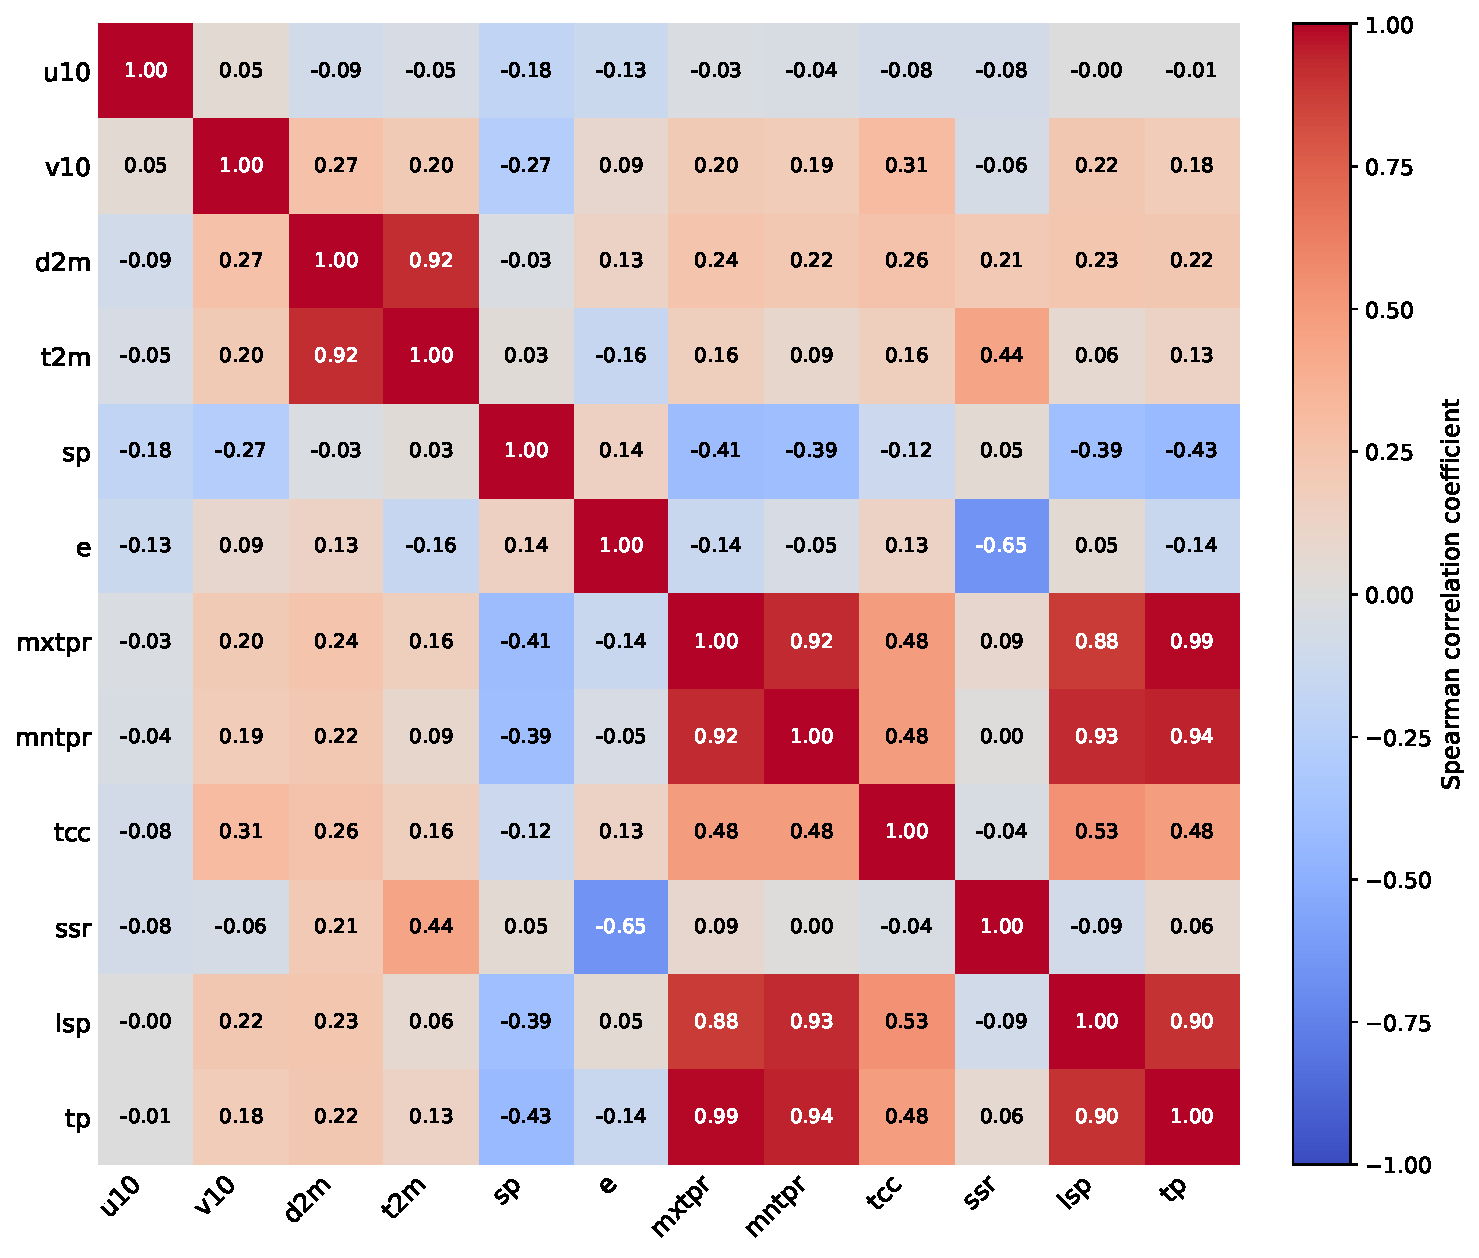
\includegraphics[width=0.7\textwidth]{train_only_spearman_heatmap.pdf}
\caption{Training-set Spearman correlation matrix among the candidate ERA5 meteorological predictors and total precipitation (tp). Correlations were computed using the training subset only to avoid information leakage}
\label{fig:Spearman}
\end{figure}

%-----------------------------------------------------
\subsection{Forecasting Models}
\label{sec:forecasting_models}

This study evaluates a set of reference, machine-learning, and deep-learning models for short-term regional precipitation forecasting, spanning different temporal representations and output formulations. Rather than presenting a single architecture as a newly proposed forecasting framework, the models are compared under a common experimental setting to examine how temporal modelling, attention, and probabilistic prediction each affect forecasting performance.

All trainable models use the seven predictors identified in Section~\ref{sec:dataset}. Each input sample is constructed from a sliding window of six consecutive 6-hourly ERA5 observations, at times $t-5$, $t-4$, $t-3$, $t-2$, $t-1$, and $t$, used to predict precipitation at the next time step, $t+1$. This window spans 30~h of historical observations, with the forecast target occurring 6~h after the final input time step. The models differ primarily in temporal representation, sequence aggregation, network depth, and deterministic versus probabilistic output formulation.


\subsubsection{Reference and Non-Recurrent Benchmark Models}
\label{sec:benchmark_models}

Persistence and climatology serve as simple reference forecasts. The persistence forecast assumes that precipitation at the next time step equals the most recently observed regional precipitation,

\begin{equation}
\hat{y}_{t+1}^{\mathrm{pers}} = y_t ,
\label{eq:persistence}
\end{equation}

where $y_t$ is the observed Dublin regional mean precipitation at the forecast origin. The climatological forecast is the mean regional precipitation over the training period,

\begin{equation}
\hat{y}_{t+1}^{\mathrm{clim}} = \frac{1}{N_{\mathrm{train}}} \sum_{i=1}^{N_{\mathrm{train}}} y_i ,
\label{eq:climatology}
\end{equation}

with $N_{\mathrm{train}}$ the number of training observations; this training-derived value is then applied unchanged to the validation and test periods.

XGBoost provides a non-sequential machine-learning benchmark. Each $6\times7$ predictor sequence is flattened into a 42-dimensional feature vector, and the model is configured with 100 boosting estimators, a learning rate of 0.05, a maximum tree depth of 6, and row and feature subsampling ratios of 0.8, producing a deterministic point estimate of regional precipitation.

A compact Transformer encoder serves as an alternative deep-learning sequence model. The seven predictors at each time step are projected into a 32-dimensional latent representation and combined with learned positional embeddings, then passed through a single encoder block with four attention heads and a feed-forward layer of 64 hidden units (dropout 0.2). Global average pooling across the temporal dimension feeds a dense output layer that produces the deterministic precipitation estimate. Given the short six-step input sequence, this compact configuration was preferred over a larger Transformer.


\subsubsection{BiLSTM and Temporal Attention Components}
\label{sec:bilstm_attention_components}

The recurrent models build on bidirectional long short-term memory (BiLSTM) networks. For an input vector $x_t$, the forward and backward hidden states are

\begin{align}
\overrightarrow{h}_t &= \overrightarrow{\mathrm{LSTM}}\left(x_t,\overrightarrow{h}_{t-1}\right), \label{eq:bilstm_forward} \\
\overleftarrow{h}_t &= \overleftarrow{\mathrm{LSTM}}\left(x_t,\overleftarrow{h}_{t+1}\right), \label{eq:bilstm_backward} \\
h_t &= \left[\overrightarrow{h}_t;\overleftarrow{h}_t\right], \label{eq:bilstm_concat}
\end{align}

with $h_t$ the concatenated bidirectional representation at time step $t$. The backward direction operates only within the historical input window available at the forecast origin: it draws on later positions inside that window, but never on observations occurring after the forecast origin itself.

For the attention-based recurrent models, additive temporal attention is applied to the hidden-state sequence $H=[h_1,h_2,\ldots,h_T]$. An unnormalized relevance score is computed for each time step,

\begin{equation}
e_t = v_a^{\top} \tanh\left(W_a h_t+b_a\right),
\label{eq:attn_score}
\end{equation}

with $W_a$, $b_a$, and $v_a$ trainable parameters. Scores are normalized across the sequence,

\begin{equation}
\alpha_t = \frac{\exp(e_t)}{\displaystyle\sum_{j=1}^{T}\exp(e_j)},
\label{eq:attn_weight}
\end{equation}

and the hidden states are aggregated into a context vector,

\begin{equation}
C = \sum_{t=1}^{T} \alpha_t h_t .
\label{eq:attn_context}
\end{equation}

The weights $\alpha_t$ thus determine how much each position in the input window contributes to the final representation.

For the deterministic BiLSTM-Attention model, the context vector maps directly to a scalar precipitation estimate,

\begin{equation}
\hat{y} = W_y C+b_y ,
\label{eq:det_output}
\end{equation}

and the model is trained with mean squared error,

\begin{equation}
\mathcal{L}_{\mathrm{MSE}} = \frac{1}{N} \sum_{i=1}^{N} \left(y_i-\hat{y}_i\right)^2 .
\label{eq:mse_loss}
\end{equation}

A BiLSTM control shares the same single BiLSTM layer (64 units), dropout rate (0.2), deterministic output, and MSE objective, but replaces attention with mean pooling over the hidden sequence,

\begin{equation}
C_{\mathrm{mean}} = \frac{1}{T} \sum_{t=1}^{T} h_t .
\label{eq:mean_pooling}
\end{equation}

The two models differ only in the temporal aggregation mechanism, allowing the effect of attention to be examined while the remaining model configuration is held fixed.


\subsubsection{Probabilistic Output Formulation}
\label{sec:probabilistic_output}

Three recurrent configurations, BU-LSTM, BU-LSTM-Attention, and Probabilistic BiLSTM-Attention, replace the deterministic scalar output with a probabilistic one, estimating both the conditional mean and variance of precipitation. Let $z_i$ denote the final latent representation for sample $i$, corresponding either to the final recurrent state or to an attention-derived context vector, depending on the architecture. Two output components are produced,

\begin{align}
\mu_i &= W_{\mu}z_i+b_{\mu}, \label{eq:prob_mu} \\
s_i &= W_s z_i+b_s, \qquad s_i=\log\sigma_i^2 , \label{eq:prob_logvar}
\end{align}

where $\mu_i$ is the predictive mean and $s_i$ the predicted log variance; the corresponding variance follows as

\begin{equation}
\sigma_i^2 = \exp(s_i),
\label{eq:prob_variance}
\end{equation}

which guarantees a positive value. Under the Gaussian assumption

\begin{equation}
y_i \mid X_i \sim \mathcal{N}\left(\mu_i,\sigma_i^2\right),
\label{eq:gaussian_assumption}
\end{equation}

these models are trained by minimizing the Gaussian negative log-likelihood. Dropping the additive constant that does not affect optimization,

\begin{equation}
\mathcal{L}_{\mathrm{NLL}} = \frac{1}{N} \sum_{i=1}^{N} \left[\frac{1}{2}\exp(-s_i)\left(y_i-\mu_i\right)^2 + \frac{1}{2}s_i\right].
\label{eq:nll_loss}
\end{equation}

The first term weighs the prediction error against the estimated variance; the second penalizes unnecessarily large variance estimates. The network thus learns predictive mean and dispersion jointly, rather than a single point estimate. A nominal $(1-\alpha)$ prediction interval follows as

\begin{equation}
\left[\mu_i-z_{1-\alpha/2}\sigma_i,\, \mu_i+z_{1-\alpha/2}\sigma_i\right],
\label{eq:prediction_interval}
\end{equation}

with $z_{1-\alpha/2}$ the corresponding standard-normal quantile; for 95\% nominal coverage this reduces to

\begin{equation}
\left[\mu_i-1.96\sigma_i,\, \mu_i+1.96\sigma_i\right].
\label{eq:prediction_interval_95}
\end{equation}

These intervals characterize predictive dispersion under the assumed Gaussian likelihood. Because precipitation is non-negative while the Gaussian distribution is not, calibration is assessed empirically, using coverage and rainfall-regime analysis, rather than assumed from the nominal interval alone.


\subsubsection{Model Configurations}
\label{sec:model_configurations}

Table~\ref{tab:model_config} summarizes the principal models included in the main comparative evaluation, combining different sequence representations, temporal aggregation strategies, and output formulations. The BU-LSTM architecture follows the uncertainty-aware recurrent formulation introduced in our earlier work~\citep{10906190}. Here it is evaluated alongside deterministic, attention-based, and probabilistic variants within a common experiment, rather than presented as a newly proposed framework.

\begin{table}[htbp]
\centering
\caption{Configuration of the forecasting models evaluated in this study.}
\label{tab:model_config}

\small
\setlength{\tabcolsep}{5pt}
\renewcommand{\arraystretch}{1.15}

\resizebox{\textwidth}{!}{%
\begin{tabular}{@{}lllll@{}}
\hline
\textbf{Model} &
\textbf{Sequence representation} &
\textbf{Temporal aggregation} &
\textbf{Output} &
\textbf{Objective} \\
\hline

Persistence &
Most recent observation &
Not applicable &
$\hat{y}$ &
Not trained \\

Climatology &
Training-period mean &
Not applicable &
$\hat{y}$ &
Not trained \\

XGBoost &
Flattened $6\times7$ input &
Gradient-boosted trees &
$\hat{y}$ &
Squared-error regression \\

Transformer &
1 encoder block, $d_{\mathrm{model}}=32$, 4 heads &
Global average pooling &
$\hat{y}$ &
MSE \\

BiLSTM &
1$\times$BiLSTM(64), dropout 0.2 &
Mean pooling &
$\hat{y}$ &
MSE \\

BiLSTM-Attention &
1$\times$BiLSTM(64), dropout 0.2 &
Additive attention (64 units) &
$\hat{y}$ &
MSE \\

BU-LSTM &
2$\times$BiLSTM(50), dropout 0.3 &
Final recurrent representation &
$\mu,\log\sigma^2$ &
Gaussian NLL \\

BU-LSTM-Attention &
3$\times$BiLSTM(64), dropout 0.2 &
Additive attention (64 units) &
$\mu,\log\sigma^2$ &
Gaussian NLL \\

Prob. BiLSTM-Attention &
1$\times$BiLSTM(64), dropout 0.2 &
Additive attention (64 units) &
$\mu,\log\sigma^2$ &
Gaussian NLL \\

\hline
\end{tabular}%
}
\end{table}

The BU-LSTM comprises two stacked BiLSTM layers with 50 units: the first returns the full hidden-state sequence, and the second produces the final bidirectional representation. A dropout rate of 0.3 follows each recurrent layer, and the final representation feeds a two-unit output layer for $\mu$ and $\log\sigma^2$.

BU-LSTM-Attention instead uses three stacked BiLSTM layers with 64 units and dropout 0.2 after each layer; all three retain the full temporal sequence, after which additive attention produces the context vector that feeds the same two probabilistic outputs, trained with Gaussian NLL. Because BU-LSTM and BU-LSTM-Attention differ in depth and hidden dimension as well as in the presence of attention, their performance gap cannot be attributed to attention alone.

A more direct test of output formulation comes from comparing the deterministic BiLSTM-Attention and Probabilistic BiLSTM-Attention models, which share the same single BiLSTM layer (64 units), dropout (0.2), and attention mechanism, and differ only in the final layer: a scalar output trained with MSE versus $\mu,\log\sigma^2$ trained with Gaussian NLL. This pairing isolates the effect of the probabilistic formulation while holding the encoder and attention architecture fixed.

To separate architecture effects from output-formulation effects more directly, a deterministic diagnostic control was also evaluated: it retains BU-LSTM-Attention's three-layer BiLSTM(64) backbone, dropout 0.2, and additive attention, but replaces the probabilistic output with a scalar one trained on MSE. As this control serves a specific diagnostic purpose rather than functioning as a primary forecasting benchmark, it is omitted from Table~\ref{tab:model_config}; its results are reported alongside the corresponding diagnostic analyses in Section~\ref{sec:diagnostic_analysis}.

Optimization settings, the early-stopping procedure, the chronological train--validation--test protocol, random-seed experiments, and evaluation metrics are described separately in Section~\ref{sec:experimental_setup}.


%---------------------------------------------------------
\subsection{Experimental Setup and Evaluation}
\label{sec:experimental_setup}

The deep-learning models were implemented in TensorFlow/Keras and trained using the Adam optimizer. Unless otherwise specified by the model architecture, the learning rate was set to 0.001, the batch size to 32, and the maximum number of training epochs to 30. Validation loss was monitored during training, and early stopping was applied when no improvement was observed for ten consecutive epochs. The model weights associated with the lowest validation loss were restored before evaluation. Deterministic neural networks were trained using mean squared error, whereas the probabilistic models were optimized using Gaussian negative log-likelihood. Hyperparameter settings were fixed before evaluation on the test set.

Point forecast accuracy was assessed using root mean squared error (RMSE), mean absolute error (MAE), and the coefficient of determination ($R^2$). For observations $y_i$ and corresponding predictions $\hat{y}_i$, RMSE and MAE are defined as

\begin{equation}
\mathrm{RMSE}
=
\sqrt{
\frac{1}{N}
\sum_{i=1}^{N}
\left(y_i-\hat{y}_i\right)^2
},
\label{eq:rmse}
\end{equation}

\begin{equation}
\mathrm{MAE}
=
\frac{1}{N}
\sum_{i=1}^{N}
\lvert y_i-\hat{y}_i\rvert,
\label{eq:mae}
\end{equation}

while $R^2$ is calculated as

\begin{equation}
R^2
=
1-
\frac{
\sum_{i=1}^{N}
\left(
y_i-\hat{y}_i
\right)^2
}{
\sum_{i=1}^{N}
\left(
y_i-\bar{y}
\right)^2
},
\label{eq:r2}
\end{equation}

where $\bar{y}$ denotes the mean observed precipitation. RMSE places greater weight on large forecast errors, while MAE provides a complementary measure that is less sensitive to individual large deviations. Because precipitation is strongly skewed and contains a large proportion of low or zero values, these metrics were considered jointly when comparing model performance.

To examine whether forecasting performance varied with precipitation intensity, the test set was also evaluated across several rainfall regimes. Wet conditions were defined as observations with precipitation greater than 0~mm. Upper-tail rainfall events were identified using the 90th, 95th, and 97.5th percentiles (Q90, Q95, and Q97.5) of the precipitation distribution in the training set. Using training-derived thresholds ensured that information from the test period was not used to define the rainfall regimes. Heavy rainfall refers to observations exceeding the training-derived Q95 threshold, which was 0.5740~mm in the present dataset.

Rainfall occurrence was further evaluated at several fixed precipitation thresholds to examine changes in event-detection skill as rainfall intensity increased. Continuous observations and predictions were converted into binary events using thresholds of $>0$, $\geq0.1$, $\geq0.5$, and $\geq1.0$~mm. The zero threshold distinguishes any recorded rainfall from dry conditions, while the positive thresholds represent progressively stronger rainfall events. For each threshold, observed and predicted events were classified as true positives (TP), false positives (FP), false negatives (FN), and true negatives (TN).

Event detection was evaluated using accuracy, precision, probability of detection (POD), F1 score, critical success index (CSI), and false alarm ratio (FAR). POD is equivalent to recall and represents the proportion of observed rainfall events that were correctly identified. CSI accounts for both missed events and false alarms and is defined as

\begin{equation}
\mathrm{CSI}
=
\frac{\mathrm{TP}}
{\mathrm{TP}+\mathrm{FP}+\mathrm{FN}},
\label{eq:csi}
\end{equation}

while FAR is given by

\begin{equation}
\mathrm{FAR}
=
\frac{\mathrm{FP}}
{\mathrm{TP}+\mathrm{FP}}.
\label{eq:far}
\end{equation}

Accuracy, precision, POD, and F1 score were calculated using their standard definitions. The threshold analysis was performed directly on the saved test predictions and therefore did not require additional model training.

For models producing predictive distributions, probabilistic performance was evaluated using Gaussian negative log-likelihood (NLL), continuous ranked probability score (CRPS), empirical prediction interval coverage, and mean prediction interval width. NLL evaluates the likelihood assigned to the observed precipitation under the predicted distribution, while CRPS measures the agreement between the full predictive distribution and the observation. Lower values indicate better performance for both metrics. Empirical coverage was calculated for nominal 90\% and 95\% prediction intervals and compared with the corresponding nominal levels. Mean interval width was reported together with coverage because high coverage can result either from well-calibrated uncertainty estimates or from intervals that are unnecessarily wide.

The Gaussian predictive distribution is unbounded, so some prediction intervals may extend below 0~mm even though precipitation is non-negative. The proportion of forecasts with a lower bound below 0~mm for the nominal 95\% prediction interval was calculated as an additional diagnostic. This measure was reported separately from the calibration metrics because it reflects a limitation of the Gaussian distributional assumption rather than calibration performance itself.

The robustness of model performance was examined using repeated runs with different random seeds. Six models were included in this analysis: XGBoost, BiLSTM, BiLSTM-Attention, BU-LSTM, BU-LSTM-Attention, and Probabilistic BiLSTM-Attention. Five fixed random seeds were used: 42, 123, 7, 2024, and 99. The data partitions, preprocessing procedure, model architecture, and training settings were kept unchanged across runs. RMSE, MAE, and $R^2$ were recorded for each seed, and the mean and standard deviation across the five runs were used to assess the robustness of model performance. For BU-LSTM, BU-LSTM-Attention, and Probabilistic BiLSTM-Attention, NLL, CRPS, and empirical 95\% interval coverage were also calculated for each run.

A paired block-bootstrap analysis was additionally conducted to assess the uncertainty in the RMSE difference between BiLSTM-Attention and XGBoost while retaining the paired structure of their test predictions and accounting for temporal dependence in the time series. The comparison was performed separately for the complete test set, wet observations, and the heavy-rainfall subset defined by the training-derived Q95 threshold. The same resampled observations were used for both models within each bootstrap replicate, and the RMSE difference was defined as

\begin{equation}
\Delta \mathrm{RMSE}
=
\mathrm{RMSE}_{\mathrm{BiLSTM\text{-}Attention}}
-
\mathrm{RMSE}_{\mathrm{XGBoost}}.
\label{eq:bootstrap_delta_rmse}
\end{equation}

Negative values of $\Delta\mathrm{RMSE}$ indicate lower RMSE for BiLSTM-Attention, whereas positive values indicate lower RMSE for XGBoost. The resulting bootstrap distribution was used to derive 95\% confidence intervals for the difference in RMSE between the two models.

All evaluation metrics were calculated after transforming the model outputs back to the original precipitation unit of millimetres. The same evaluation procedure was applied to the saved predictions from each model so that the reported results were directly comparable across model configurations.
%---------------------------------------------------
\subsection{Model Interpretability and Diagnostic Analysis}
\label{sec:diagnostic_analysis}

Model interpretation was examined using SHAP-based feature attribution and feature ablation. These analyses provide different views of predictor relevance. SHAP describes how the fitted model distributes its predictions among the available inputs, whereas feature ablation measures the change in predictive performance when individual predictors are removed. An additional deterministic control was also used to examine the effect of the probabilistic output formulation within the deeper BU-LSTM-Attention architecture.

\subsubsection{SHAP-Based Feature Attribution}
\label{sec:shap}

SHAP analysis was applied to the BiLSTM-Attention model to examine how the selected meteorological predictors contributed to its precipitation forecasts. SHAP provides feature attributions based on Shapley values and assigns each input a contribution relative to the expected model output \citep{lundberg2017unified}. For a feature $j$ drawn from the complete feature set $\mathcal{N}$, the corresponding Shapley value is defined as

\begin{equation}
\label{eq:shapley}
\phi_j =
\sum_{S \subseteq \mathcal{N}\setminus\{j\}}
\frac{\lvert S\rvert!\left(\lvert\mathcal{N}\rvert-\lvert S\rvert-1\right)!}
{\lvert\mathcal{N}\rvert!}
\left[v(S\cup\{j\})-v(S)\right].
\end{equation}

where $S$ denotes a subset of the available inputs and $v(S)$ represents the model output associated with that subset. The weighting term averages the marginal contribution of feature $j$ over the possible feature orderings \citep{rozemberczki2022shapley}.

Attributions were computed using the model-agnostic permutation implementation of \texttt{shap.Explainer}. A gradient-based explainer was not used owing to repeated compatibility issues with Keras 3 in the software environment used for the experiments. The explainer operated on a prediction wrapper that reshaped the flattened inputs to their original temporal form and transformed the model output back to millimetres before evaluation. The resulting SHAP values are therefore expressed in millimetres. The background distribution consisted of 50 training windows sampled at random without replacement, while 100 test windows were sampled in the same manner for attribution analysis. A fixed random seed of 42 was used for this sampling procedure. For the six time steps and seven predictors, the model-agnostic explainer operated on 42 input dimensions and used the permutation algorithm with a maximum of $2M+1$ evaluations, where $M=42$.

The sequential input contains both predictor and temporal dimensions. SHAP values were therefore reshaped back to the original $T\times F$ structure after attribution, retaining the contribution of each meteorological variable at each of the six input times. Global importance for predictor $j$ was summarized using the mean absolute SHAP value across the evaluated samples and time steps,

\begin{equation}
I_j =
\frac{1}{NT}
\sum_{i=1}^{N}
\sum_{t=1}^{T}
\lvert
\phi_{i,j,t}
\rvert,
\label{eq:global_shap}
\end{equation}

where $\phi_{i,j,t}$ denotes the attribution of predictor $j$ at input time $t$ for sample $i$. Temporal importance was calculated separately for each position in the input sequence,

\begin{equation}
I_{j,t} =
\frac{1}{N}
\sum_{i=1}^{N}
\lvert
\phi_{i,j,t}
\rvert.
\label{eq:temporal_shap}
\end{equation}

The global measure summarizes the overall attribution of each meteorological variable, while the temporal measure retains changes in attribution across the historical input window. Signed SHAP values were also examined to determine whether particular predictor values were associated with increases or decreases in the model output relative to its baseline prediction.

SHAP values are interpreted here as model-specific attributions rather than causal effects or direct measures of feature necessity. This distinction is important when predictors contain overlapping information. Spearman correlation describes the marginal association between individual predictors and precipitation, SHAP characterizes attribution within the fitted model, and the feature-ablation analysis evaluates how predictive performance changes when a predictor is removed.

\subsubsection{Feature Ablation Analysis}
\label{sec:feature_ablation}

A leave-one-feature-out experiment was conducted for BU-LSTM-Attention to assess the predictive contribution of the seven selected variables. The full model contained mxtpr, mntpr, lsp, tcc, v10, sp, and d2m. Seven additional models were trained by removing one predictor at a time while retaining the same network structure and training procedure. Performance was evaluated using RMSE, MAE, and $R^2$.

The effect of removing predictor $j$ was summarized by the change in RMSE relative to the full model,

\begin{equation}
\Delta \mathrm{RMSE}_j
=
\mathrm{RMSE}_{-j}
-
\mathrm{RMSE}_{\mathrm{full}},
\label{eq:delta_rmse}
\end{equation}

where $\mathrm{RMSE}_{-j}$ is the test RMSE after excluding predictor $j$. Positive values indicate an increase in error after removal, whereas negative values indicate a lower RMSE for that particular run. Small negative differences were not interpreted as evidence that a predictor was detrimental, because correlated predictors and stochastic model training can produce modest changes in either direction.

The initial ablation experiment evaluated all seven predictors using a common random seed. A targeted robustness analysis was then carried out for tcc and mxtpr, which showed contrasting behaviour in the initial experiment. Five seeds, 42, 123, 7, 2024, and 99, were used. For each seed, the ablated model was compared with the full BU-LSTM-Attention model trained using the same seed, and the resulting RMSE differences were summarized across the five runs. Matching the random seed between the full and ablated configurations reduces variation associated with model initialization when assessing the effect of feature removal.

The ablation results were considered together with the Spearman and SHAP analyses, but the three measures were not expected to produce identical rankings. Spearman correlation measures marginal association with the target, SHAP measures attribution within the fitted model, and ablation measures the change in predictive performance when a predictor is removed. Differences among these measures can arise when several variables contain redundant or strongly related information.

\subsubsection{Matched Deterministic Diagnostic Control}
\label{sec:deterministic_control}

A matched deterministic control was used to examine the effect of the probabilistic output formulation within the BU-LSTM-Attention architecture. The control retained the same three stacked BiLSTM layers with 64 units, dropout rate of 0.2, and additive temporal attention used by BU-LSTM-Attention. The two probabilistic outputs were replaced by a single deterministic precipitation output, and the network was trained using mean squared error instead of Gaussian negative log-likelihood.

The recurrent backbone and attention mechanism were therefore held fixed, while the output formulation and training objective were changed. The deterministic control and BU-LSTM-Attention were compared using the same point forecast metrics. This configuration was treated as a diagnostic experiment rather than as an additional model in the main benchmark comparison.

%---------------------------------------------------
\section{Results}
\label{sec:results}

The results are presented from three complementary perspectives. First, the overall forecasting performance and its sensitivity to random initialization are examined across the evaluated models. Second, performance is assessed under wet and heavy-rainfall conditions, together with the quality of the probabilistic forecasts. Finally, SHAP attribution and feature-ablation experiments are used to examine how the selected predictors contribute to the fitted models.

%----------------------------------------------------
\subsection{Overall Forecasting Performance and Robustness}
\label{sec:overall_results}

All trainable models improved substantially over the simple reference forecasts on the test set. In the single-run evaluation, persistence produced an RMSE of 0.3282~mm and climatology an RMSE of 0.2737~mm, compared with 0.2591~mm for the Transformer, 0.2487~mm for BU-LSTM, 0.2481~mm for Probabilistic BiLSTM-Attention, 0.2464~mm for BU-LSTM-Attention, 0.2438~mm for XGBoost, and 0.2428~mm for BiLSTM-Attention. The corresponding $R^2$ values ranged from negative values for the two reference forecasts to 0.2119 for BiLSTM-Attention.

Because the differences among the leading trainable models were small, the main comparison was based on five fixed random seeds rather than on a single run. Table~\ref{tab:seed_stability} summarizes the resulting point-forecast metrics. BiLSTM-Attention achieved the lowest mean RMSE, $0.2429\pm0.0010$~mm, followed by XGBoost at $0.2439\pm0.0002$~mm and the BiLSTM control at $0.2447\pm0.0012$~mm. BU-LSTM-Attention and BU-LSTM produced very similar mean RMSE values of 0.2469~mm, while Probabilistic BiLSTM-Attention had the largest mean RMSE among the six models included in the multi-seed experiment at $0.2488\pm0.0017$~mm.

\begin{table}[htbp]
\centering
\caption{Point-forecast performance across five fixed random seeds. Values are reported as mean $\pm$ standard deviation.}
\label{tab:seed_stability}
\small
\setlength{\tabcolsep}{4pt}
\begin{tabular}{lccc}
\hline
\textbf{Model} & \textbf{RMSE (mm)} & \textbf{MAE (mm)} & \textbf{$R^2$} \\
\hline
BiLSTM-Attention
& $0.2429 \pm 0.0010$
& $0.1182 \pm 0.0021$
& $0.2117 \pm 0.0063$ \\

XGBoost
& $0.2439 \pm 0.0002$
& $0.1191 \pm 0.0005$
& $0.2049 \pm 0.0016$ \\

BiLSTM
& $0.2447 \pm 0.0012$
& $0.1183 \pm 0.0017$
& $0.2001 \pm 0.0079$ \\

BU-LSTM-Attention
& $0.2469 \pm 0.0021$
& $0.1202 \pm 0.0025$
& $0.1851 \pm 0.0137$ \\

BU-LSTM
& $0.2470 \pm 0.0013$
& $0.1191 \pm 0.0016$
& $0.1849 \pm 0.0085$ \\

Probabilistic BiLSTM-Attention
& $0.2488 \pm 0.0017$
& $0.1216 \pm 0.0037$
& $0.1724 \pm 0.0112$ \\
\hline
\end{tabular}
\end{table}

The five-seed RMSE distributions are shown in Fig.~\ref{fig:seed_rmse}. The difference between BiLSTM-Attention and XGBoost was small, amounting to approximately 0.0010~mm in mean RMSE. The matched no-attention control also remained close to BiLSTM-Attention, although temporal attention reduced the mean RMSE from 0.2447 to 0.2429~mm under the otherwise identical one-layer BiLSTM configuration. The improvement associated with attention was therefore modest relative to the overall level of forecast error.

\begin{figure}[htbp]
    \centering
    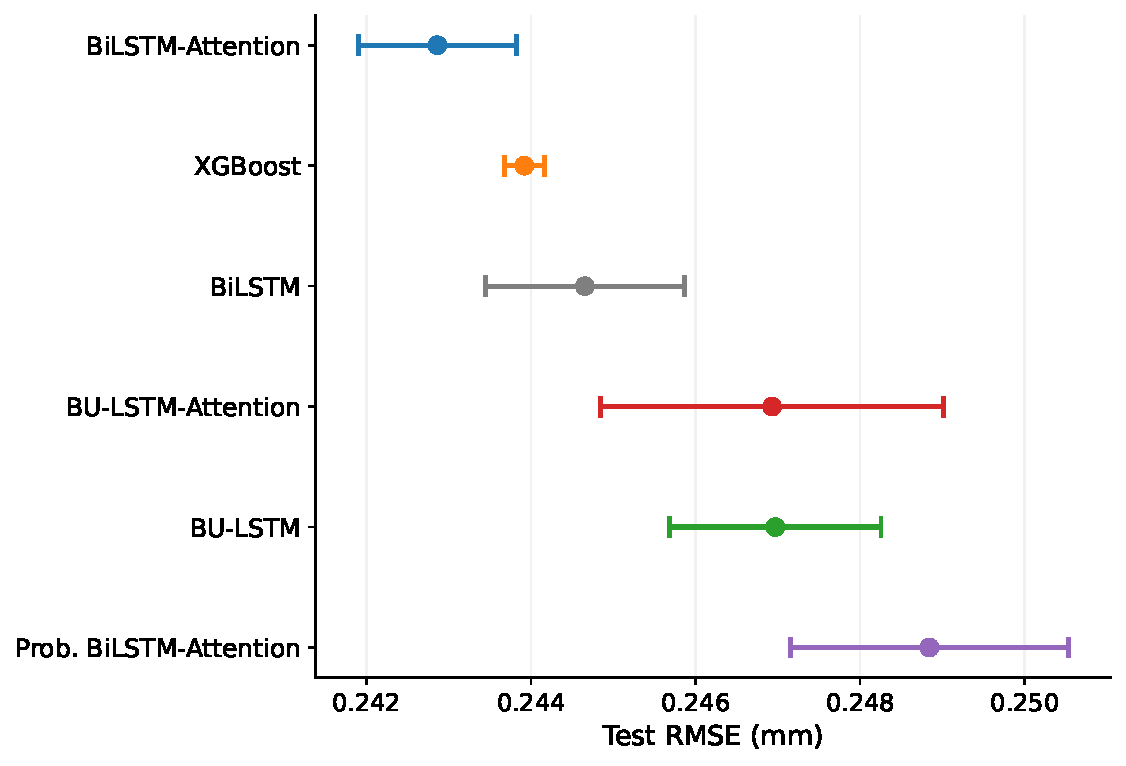
\includegraphics[width=0.78\textwidth]{fig1_5seed_rmse.pdf}
    \caption{Test RMSE across five fixed random seeds for the principal forecasting models. Points show the mean and error bars show one standard deviation}
    \label{fig:seed_rmse}
\end{figure}

A paired block-bootstrap comparison was also performed for BiLSTM-Attention and XGBoost. For the complete test set, the RMSE difference defined as BiLSTM-Attention minus XGBoost was $-0.0009$~mm, with a 95\% confidence interval from $-0.0049$ to 0.0033~mm. For wet samples, the corresponding difference was $-0.0003$~mm, with a 95\% confidence interval from $-0.0046$ to 0.0043~mm. Both intervals included zero, indicating that the small overall and wet-condition RMSE differences between these two models were not clearly distinguishable in the bootstrap analysis.

%----------------------------------------------------
\subsection{Performance Across Rainfall Regimes}
\label{sec:regime_results}

Forecast errors increased substantially when the evaluation was restricted to wetter and heavier precipitation. Of the 3,939 test samples, 3,228 contained precipitation above 0~mm, while 238 exceeded the training-derived 95th-percentile threshold of 0.5740~mm. Figure~\ref{fig:stratified_rmse} compares RMSE for the full test set, wet samples, and heavy-rainfall samples.

For all test samples, BiLSTM-Attention and XGBoost achieved RMSE values of 0.2428 and 0.2438~mm, respectively. Their performance remained almost identical for wet conditions, with RMSE values of 0.2672 and 0.2674~mm. A different ordering emerged for heavy rainfall. XGBoost produced the lowest RMSE at 0.8417~mm, followed by BiLSTM-Attention at 0.8784~mm and BU-LSTM-Attention at 0.8859~mm. BU-LSTM and Probabilistic BiLSTM-Attention reached 0.9146 and 0.8980~mm, respectively. The deterioration was also reflected in strongly negative $R^2$ values for all models within the heavy-rainfall subset.

\begin{figure}[htbp]
    \centering
    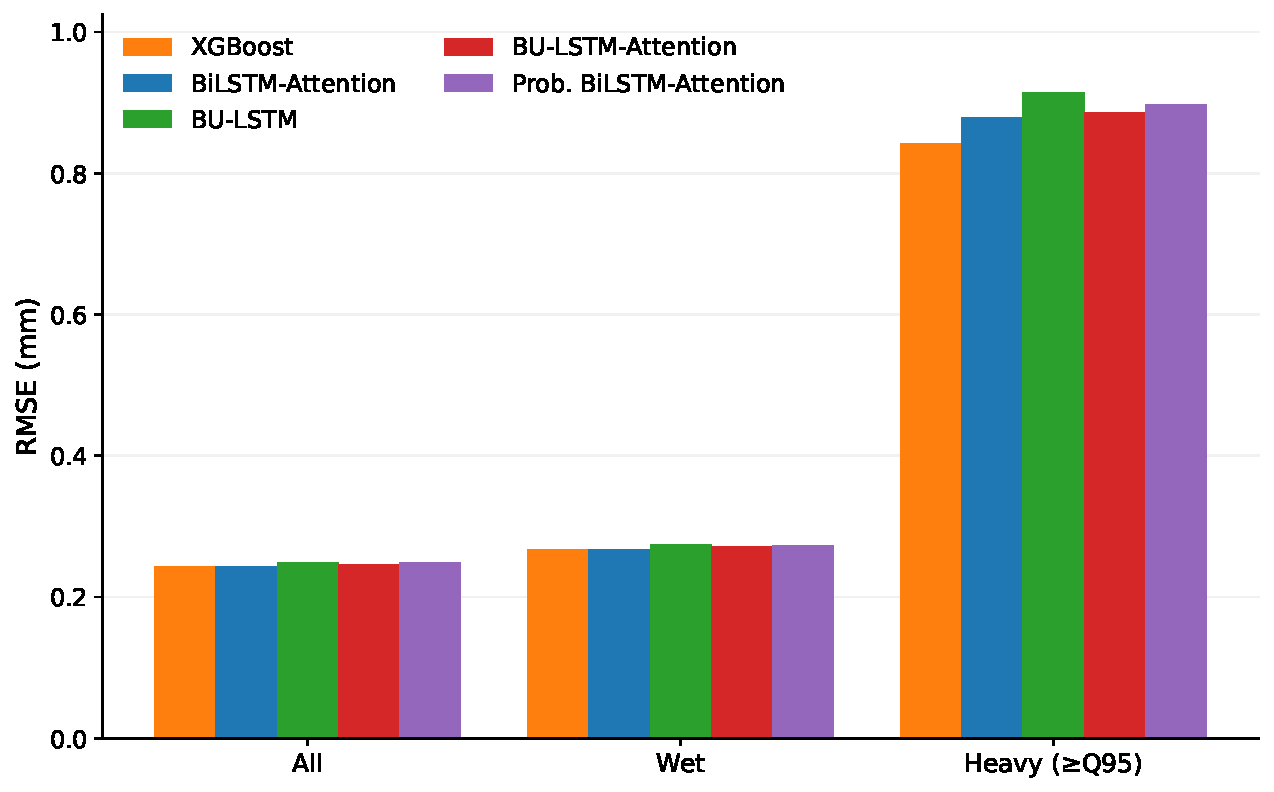
\includegraphics[width=0.78\textwidth]{fig2_stratified_rmse.pdf}
    \caption{Test RMSE for all samples, wet samples, and heavy-rainfall samples exceeding the training-derived 95th-percentile precipitation threshold}
    \label{fig:stratified_rmse}
\end{figure}

The block-bootstrap analysis supported the change in model ordering under heavy rainfall. For samples above the 95th-percentile threshold, the RMSE difference between BiLSTM-Attention and XGBoost was 0.0368~mm, with a 95\% confidence interval from 0.0190 to 0.0554~mm. The interval remained entirely above zero, indicating a consistent RMSE advantage for XGBoost within this subset.

The same pattern became more pronounced as the precipitation threshold increased. Using training-derived thresholds, XGBoost achieved RMSE values of 0.6265, 0.8417, and 1.1231~mm for the Q90, Q95, and Q97.5 subsets, compared with 0.6527, 0.8784, and 1.1696~mm for BiLSTM-Attention. Thus, the overall advantage of BiLSTM-Attention did not extend to the upper tail of the precipitation distribution.

The event-based analysis showed a similar loss of discrimination at higher rainfall thresholds. At a threshold of 0.1~mm, representing 21.68\% of the test observations, BiLSTM-Attention achieved the highest CSI at 0.4174, followed closely by XGBoost at 0.4112, BU-LSTM-Attention at 0.4049, and Probabilistic BiLSTM-Attention at 0.4044. At 0.5~mm, only 7.31\% of observations were classified as events, and CSI decreased sharply. Persistence and XGBoost retained CSI values of 0.1660 and 0.1127, while BiLSTM-Attention reached 0.0208 and the remaining recurrent probabilistic models produced no positive detections. At 1.0~mm, which represented 2.31\% of the test set, CSI was close to zero for all models. These results show that event-detection skill decreased rapidly as the rainfall threshold increased.

%----------------------------------------------------
\subsection{Probabilistic Forecast Performance}
\label{sec:probabilistic_results}

The three probabilistic recurrent models produced similar uncertainty scores when averaged across five random seeds. BU-LSTM achieved the lowest mean NLL and CRPS, with values of $-0.4874\pm0.0233$ and $0.0943\pm0.0013$, respectively. BU-LSTM-Attention produced an NLL of $-0.4675\pm0.0758$ and a CRPS of $0.0950\pm0.0014$, while Probabilistic BiLSTM-Attention obtained $-0.4356\pm0.1190$ and $0.0964\pm0.0032$. Mean empirical coverage of the nominal 95\% prediction intervals was 0.9559 for BU-LSTM, 0.9581 for BU-LSTM-Attention, and 0.9568 for Probabilistic BiLSTM-Attention. These probabilistic results are summarized in Table~\ref{tab:probabilistic_results}.

\begin{table}[htbp]
\centering
\caption{Probabilistic performance across five fixed random seeds. Values are reported as mean $\pm$ standard deviation. Cov$_{95}$ denotes empirical coverage of the nominal 95\% prediction interval.}
\label{tab:probabilistic_results}

\small
\setlength{\tabcolsep}{4pt}

\begin{tabular}{@{}lccc@{}}
\hline
\textbf{Model} &
\textbf{NLL} &
\textbf{CRPS (mm)} &
\textbf{Cov$_{95}$} \\
\hline

BU-LSTM &
$-0.4874 \pm 0.0233$ &
$0.0943 \pm 0.0013$ &
$0.9559 \pm 0.0031$ \\

BU-LSTM-Attention &
$-0.4675 \pm 0.0758$ &
$0.0950 \pm 0.0014$ &
$0.9581 \pm 0.0033$ \\

Prob. BiLSTM-Attention &
$-0.4356 \pm 0.1190$ &
$0.0964 \pm 0.0032$ &
$0.9568 \pm 0.0077$ \\

\hline
\end{tabular}
\end{table}

The near-nominal coverage obtained over the complete test set did not persist under stronger rainfall conditions. As shown in Fig.~\ref{fig:prob_coverage}, empirical 95\% coverage remained between approximately 0.94 and 0.95 for wet samples, but fell sharply for the Q95 heavy-rainfall subset. Coverage decreased to 0.5000 for BU-LSTM-Attention, 0.4958 for Probabilistic BiLSTM-Attention, and 0.4370 for BU-LSTM. At the Q97.5 threshold, the corresponding values declined further to 0.2830, 0.3113, and 0.1887.

\begin{figure}[htbp]
    \centering
    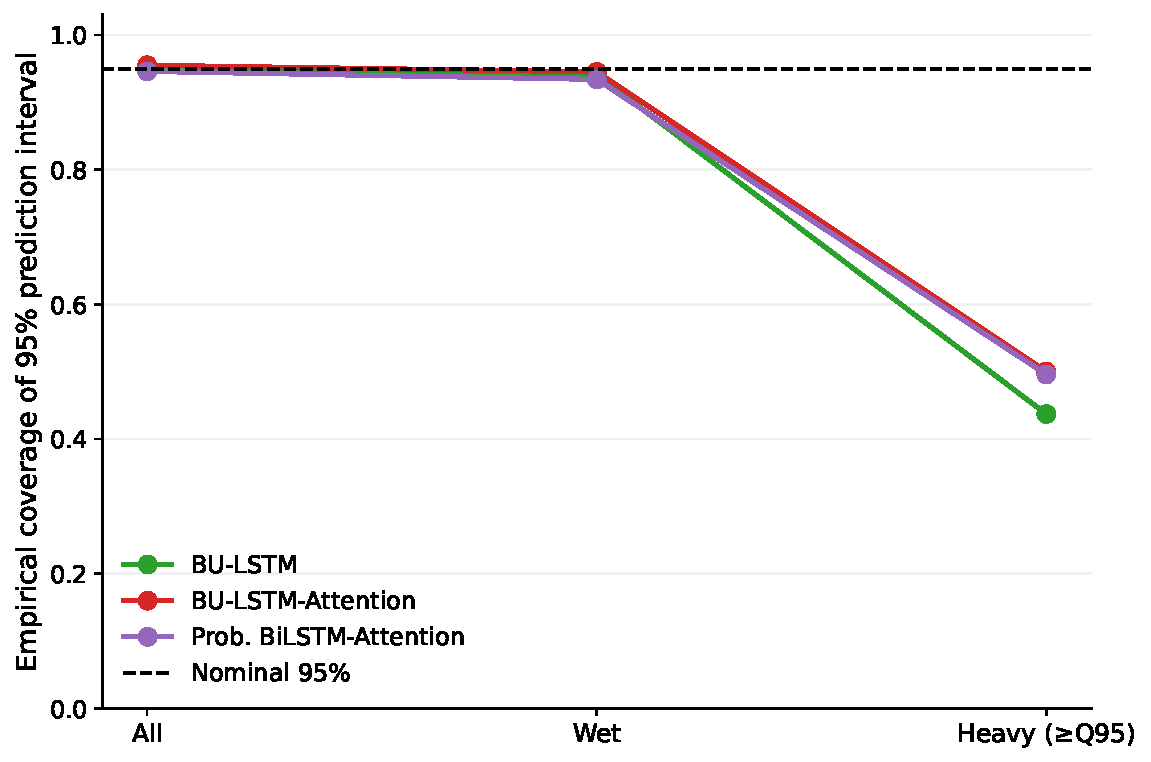
\includegraphics[width=0.78\textwidth]{fig3_probabilistic_coverage.pdf}
    \caption{Empirical coverage of the nominal 95\% prediction interval for all, wet, and heavy-rainfall samples}
    \label{fig:prob_coverage}
\end{figure}

Prediction intervals widened as rainfall intensity increased, but the increase was insufficient to maintain nominal coverage in the upper tail. For example, BU-LSTM-Attention had a mean 95\% interval width of 0.7473~mm over the full test set and 1.4459~mm for the Q95 subset, yet heavy-rainfall coverage was only 0.5000. All three Gaussian models also produced lower 95\% interval bounds below 0~mm for every test sample in the single-run diagnostic. This result reflects the mismatch between the unbounded Gaussian predictive distribution and the non-negative support of precipitation.

A cost in point accuracy was also observed when the deterministic BiLSTM-Attention architecture was converted to a probabilistic formulation. Across five seeds, mean RMSE increased from 0.2429~mm for BiLSTM-Attention to 0.2488~mm for Probabilistic BiLSTM-Attention, corresponding to an increase of approximately 2.5\%. The probabilistic formulation therefore provided distributional information and near-nominal overall coverage, but did not improve point-forecast accuracy.

%----------------------------------------------------
\subsection{SHAP-Based Feature Attribution}
\label{sec:shap_results}

SHAP analysis was performed on the representative seed-42 BiLSTM-Attention model. Its test RMSE was 0.2428~mm, close to the five-seed mean of $0.2429\pm0.0010$~mm. Global mean absolute SHAP values ranked total cloud cover as the most influential predictor at 0.0089~mm, followed by the 10-m meridional wind component at 0.0086~mm, surface pressure at 0.0083~mm, and minimum total precipitation rate at 0.0081~mm. Dew-point temperature, maximum precipitation rate, and large-scale precipitation had lower global mean absolute SHAP values of approximately 0.0034, 0.0029, and 0.0018~mm, respectively.

The temporal distribution in Fig.~\ref{fig:temporal_shap} shows that attribution was concentrated toward the most recent part of the six-step input window. At the current input time, the largest mean absolute SHAP value was associated with minimum precipitation rate, at approximately 0.041~mm, followed by total cloud cover at 0.035~mm, surface pressure at 0.030~mm, and v10 at 0.028~mm. Attribution was generally smaller at earlier input times, although the magnitude and temporal pattern differed among predictors.

\begin{figure}[htbp]
    \centering
    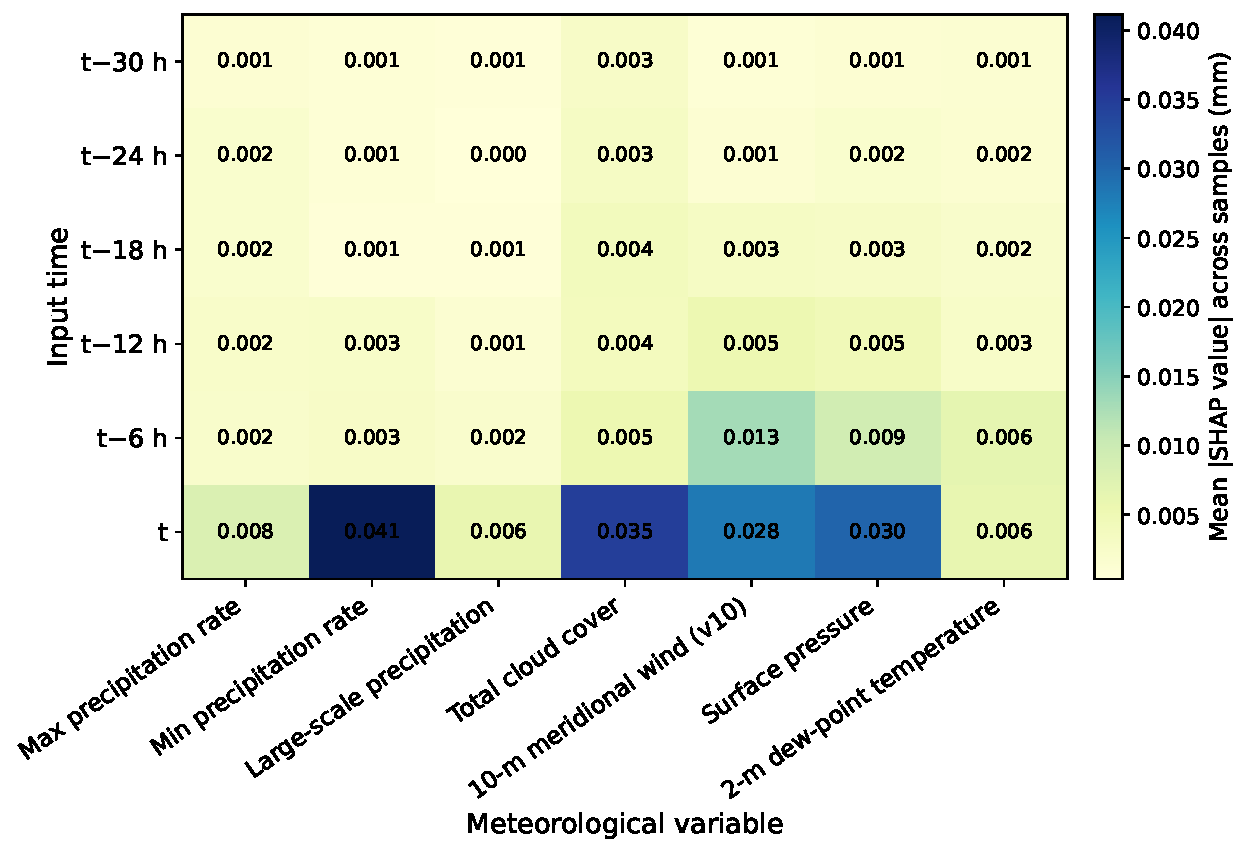
\includegraphics[width=0.82\textwidth]{fig5_temporal_shap.pdf}
    \caption{Mean absolute SHAP values for the seven meteorological predictors across the six input times}
    \label{fig:temporal_shap}
\end{figure}

The signed SHAP distributions provide additional information on the direction of these contributions. Figure~\ref{fig:shap_summary} shows that high minimum precipitation-rate values at the most recent time step were associated with some of the largest positive contributions to predicted rainfall. Higher total cloud cover at the current time was also predominantly associated with positive SHAP values. Surface pressure showed the opposite pattern at the current time, with higher standardized values tending to contribute negatively and lower values tending to contribute positively. The effect of v10 varied with temporal position, illustrating that attribution to a predictor was not necessarily constant across the input window.

\begin{figure}[htbp]
    \centering
    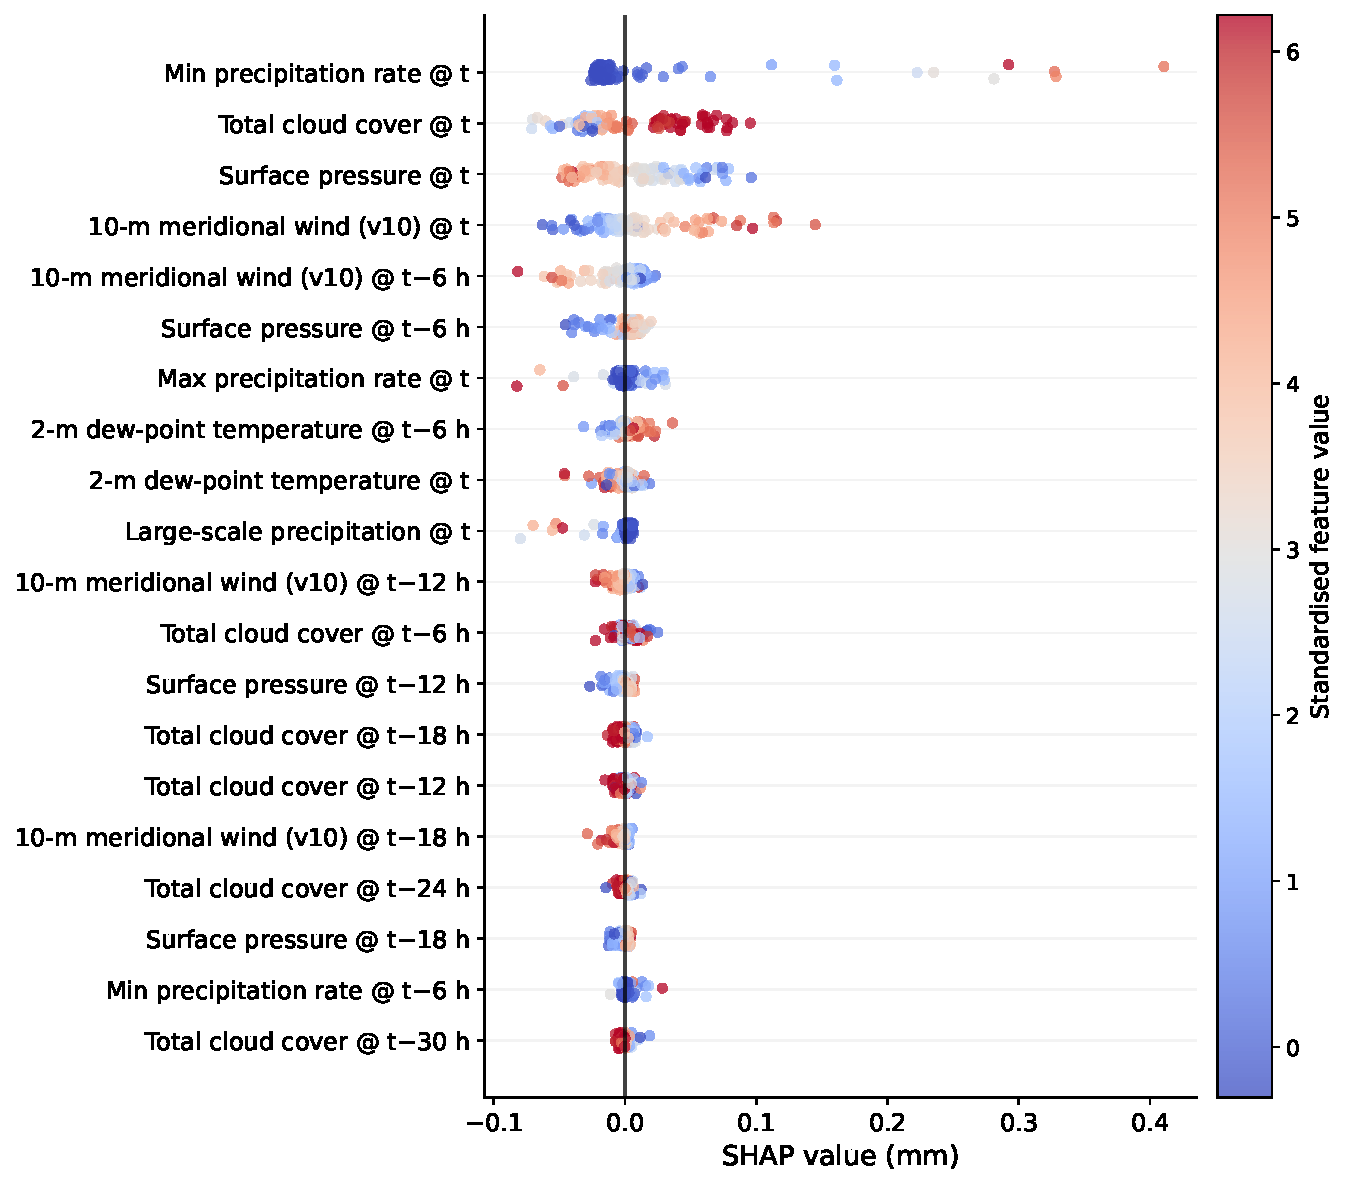
\includegraphics[width=0.82\textwidth]{fig6_shap_summary.pdf}
    \caption{SHAP value distributions for the 20 most influential predictor-time combinations in the BiLSTM-Attention model. Colour indicates the standardized predictor value}
    \label{fig:shap_summary}
\end{figure}

The SHAP ranking differed substantially from the marginal Spearman correlations used during feature screening. In particular, mxtpr had the strongest correlation with the target but relatively low global SHAP importance, whereas tcc showed only moderate marginal correlation but the largest global mean absolute SHAP value. This difference indicates that marginal association and attribution within the fitted multivariate model capture different aspects of predictor relevance.

%----------------------------------------------------
\subsection{Feature Ablation and Diagnostic Controls}
\label{sec:ablation_results}

The single-seed leave-one-feature-out experiment provided a further comparison of predictor contribution. Removing tcc produced the largest increase in RMSE, from 0.2464 to 0.2539~mm, corresponding to $\Delta\mathrm{RMSE}=+0.0075$~mm. Removing sp and v10 also increased RMSE, although by smaller amounts of 0.0023 and 0.0016~mm. In contrast, removing lsp, d2m, mntpr, or mxtpr resulted in small reductions in RMSE in that individual run.

The two most informative cases were examined across five seeds. Figure~\ref{fig:feature_ablation} shows that the full BU-LSTM-Attention model had a mean RMSE of $0.2469\pm0.0021$~mm. Removing tcc increased the mean RMSE to $0.2508\pm0.0035$~mm, with a mean paired change of $+0.0039$~mm. RMSE increased in four of the five paired seed runs. This provides evidence that tcc contributed additional predictive information beyond the other six predictors.

\begin{figure}[htbp]
    \centering
    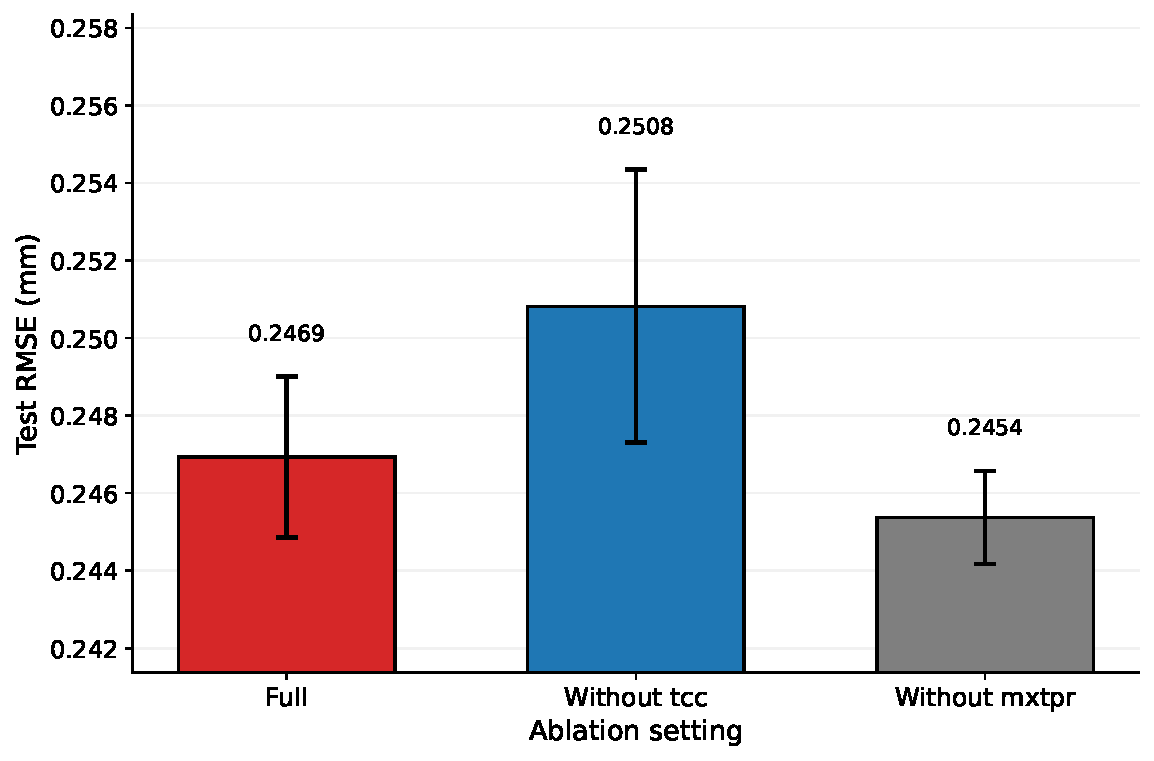
\includegraphics[width=0.78\textwidth]{feature_ablation_rmse_5seed.pdf}
    \caption{Five-seed test RMSE for the full BU-LSTM-Attention model and targeted leave-one-feature-out configurations. Error bars show one standard deviation}
    \label{fig:feature_ablation}
\end{figure}

Removing mxtpr reduced the mean RMSE to $0.2454\pm0.0012$~mm, with a mean paired change of $-0.0016$~mm. Four of the five seed runs showed a small reduction in RMSE after removal, although the magnitude was limited. Given the very high Spearman correlation between mxtpr and precipitation, together with its relatively low global SHAP importance, this result is consistent with substantial overlap between mxtpr and the other precipitation-related predictors rather than evidence that mxtpr is intrinsically detrimental.

The matched deterministic diagnostic control further clarified the effect of the probabilistic objective in the deeper BU-LSTM-Attention architecture. With the same three-layer BiLSTM-Attention backbone, the deterministic MSE model achieved an RMSE of 0.2433~mm, MAE of 0.1116~mm, and $R^2$ of 0.2091. The corresponding probabilistic BU-LSTM-Attention run produced an RMSE of approximately 0.2464~mm, MAE of 0.1174~mm, and $R^2$ of approximately 0.188. The lower point error of the matched deterministic control is consistent with the pattern observed for the one-layer BiLSTM-Attention pair, where optimizing a predictive distribution introduced a modest cost in deterministic point accuracy.
%-----------------------------------------------------
\section{Discussion}

\subsection{Overall Forecasting Performance and Model Robustness}

The results show that several machine-learning and deep-learning models achieved similar levels of performance for short-term regional precipitation forecasting over Dublin. Across five fixed random seeds, BiLSTM-Attention obtained the lowest mean RMSE of 0.2429~mm, followed closely by XGBoost at 0.2439~mm. The difference between the two models was small relative to the overall forecast error. The paired block-bootstrap analysis also showed that the RMSE differences for the complete test set and the wet subset were not clearly distinguishable, with both 95\% confidence intervals including zero. The main result is therefore not that one model consistently outperformed all alternatives, but that a relatively compact recurrent model and a tree-based machine-learning model produced comparable overall point forecasts under the same data and evaluation protocol.

The comparison between BiLSTM-Attention and BiLSTM provides a more direct assessment of the temporal attention mechanism. The attention-based model reduced the mean RMSE from 0.2447 to 0.2429~mm while the remaining architecture was kept unchanged. The improvement was consistent with a useful contribution from temporal attention, although its magnitude was modest. This result is important when interpreting architectural changes in rainfall forecasting, because differences observed in a single training run can be similar in magnitude to those caused by stochastic model initialization. The five-seed experiment therefore provides a more conservative estimate of the benefit associated with attention.

The probabilistic recurrent models did not improve deterministic point accuracy. Probabilistic BiLSTM-Attention produced a higher mean RMSE than its deterministic BiLSTM-Attention counterpart, and a similar pattern was observed for the deeper BU-LSTM-Attention architecture when compared with the matched deterministic diagnostic control. The deterministic three-layer control achieved an RMSE of 0.2433~mm, compared with approximately 0.2464~mm for the corresponding probabilistic BU-LSTM-Attention run. These differences are consistent with the models being trained for different objectives. Mean squared error directly optimizes point prediction, whereas Gaussian negative log-likelihood jointly estimates the predictive mean and variance. Probabilistic models should therefore be assessed using both point accuracy and the quality of the predictive distribution rather than point-error metrics alone.

\subsection{Performance under Heavy Rainfall and Probabilistic Reliability}

A different model ranking emerged when the analysis was restricted to heavier precipitation. BiLSTM-Attention and XGBoost performed almost identically over the full test set and the wet subset, but XGBoost achieved consistently lower RMSE at the higher precipitation thresholds. At the training-derived Q95 threshold, XGBoost obtained an RMSE of 0.8417~mm compared with 0.8784~mm for BiLSTM-Attention. The paired block-bootstrap RMSE difference between BiLSTM-Attention and XGBoost was 0.0368~mm, with a 95\% confidence interval from 0.0190 to 0.0554~mm. The interval remained above zero, providing stronger evidence of an XGBoost advantage for heavy-rainfall samples than for the test set as a whole.

This change in ranking illustrates an important limitation of aggregate forecast metrics. Most observations in the dataset correspond to dry or relatively light rainfall, so overall RMSE is dominated by the more common part of the precipitation distribution. Restricting the evaluation to Q90, Q95, and Q97.5 rainfall revealed much larger errors for all models. The event-based analysis showed the same pattern. At the 0.1~mm threshold, BiLSTM-Attention achieved a CSI of 0.4174 and several other models obtained similar values. CSI decreased sharply at 0.5~mm, and at 1.0~mm the discrimination skill of all models was close to zero. These results indicate that accurate prediction of stronger rainfall remains substantially more difficult than forecasting low and moderate precipitation.

The performance of XGBoost in the heavy-rainfall subset should not be interpreted as evidence that tree-based models were generally superior to the deep-learning models. BiLSTM-Attention remained numerically best for the overall point-forecast comparison, and the difference from XGBoost was small. The clearer advantage of XGBoost appeared only in the upper tail of the precipitation distribution. One possible explanation is that tree-based models can partition predictor space effectively without requiring the same amount of repeated examples needed to estimate complex neural-network representations. This pattern is broadly consistent with evidence that tree-based methods can match or exceed deep neural networks on tabular data, particularly under limited or imbalanced sample sizes \citep{grinsztajn2022tree}. This may be useful when high-intensity rainfall events are relatively sparse, although the present experiments do not establish the underlying mechanism directly.

The probabilistic forecasts showed a similar dependence on rainfall intensity. When evaluated over the complete test set, empirical coverage of the nominal 95\% prediction interval was close to the nominal level for all three probabilistic models, ranging from approximately 0.956 to 0.958 across the five-seed experiments. This apparently good overall calibration changed substantially when the evaluation was restricted to heavy rainfall. At Q95, empirical coverage fell to approximately 0.44 for BU-LSTM and approximately 0.50 for BU-LSTM-Attention and Probabilistic BiLSTM-Attention. Coverage decreased further at Q97.5.

Prediction intervals widened as rainfall intensity increased, but the additional width was insufficient to maintain nominal coverage for the strongest events. This result shows that acceptable calibration over the complete test distribution can conceal substantial undercoverage in a less frequent but meteorologically important regime. Reporting only overall coverage would therefore give an incomplete assessment of probabilistic forecast reliability.

The Gaussian likelihood also imposes a structural limitation on the uncertainty estimates. Precipitation is non-negative and strongly right-skewed, whereas the Gaussian distribution is symmetric and unbounded. In the single-run diagnostic, the lower bound of the nominal 95\% interval extended below 0~mm throughout the test set. Negative interval bounds do not correspond to physically meaningful precipitation and indicate a mismatch between the assumed predictive distribution and the support of the target variable. The Gaussian formulation remains useful as a probabilistic baseline, but the combination of negative lower bounds and pronounced undercoverage under heavy rainfall suggests that alternative distributions may be more appropriate for precipitation forecasting.

\subsection{Predictor Attribution and Incremental Contribution}

The SHAP analysis of the BiLSTM-Attention model provides insight into how the fitted network uses the seven selected meteorological predictors. Total cloud cover had the highest global mean absolute SHAP value, followed closely by the 10-m meridional wind component, surface pressure, and minimum total precipitation rate. The temporal analysis also showed that attribution was concentrated toward the more recent part of the six-step input sequence. At the most recent input time, minimum precipitation rate, total cloud cover, surface pressure, and v10 produced some of the largest mean absolute SHAP values. This concentration toward recent observations is consistent with the short forecast horizon considered in the study, although the strength and temporal pattern of attribution differed among predictors.

The signed SHAP distributions provide further information about the model response. Higher total cloud cover at the most recent input time was generally associated with positive contributions to predicted precipitation. Surface pressure showed a contrasting pattern, with higher values tending to contribute negatively to the model output. The influence of v10 varied across input times, indicating that the model response to individual predictors was not necessarily monotonic or temporally constant. These patterns describe associations learned by the fitted model and should not be interpreted as causal relationships between meteorological variables and precipitation.

An important finding is that the Spearman, SHAP, and feature-ablation analyses did not produce identical measures of predictor relevance. Maximum precipitation rate had a Spearman correlation of approximately 0.99 with total precipitation, making it the strongest marginally associated predictor during feature screening. Its global SHAP importance was nevertheless relatively low. Removing mxtpr from BU-LSTM-Attention also reduced the mean RMSE slightly across the targeted five-seed experiment, from 0.2469 to approximately 0.2454~mm. Four of the five paired runs showed a small improvement after its removal.

This result does not imply that mxtpr is detrimental to rainfall forecasting. Mxtpr, mntpr, and lsp are strongly related precipitation variables and therefore contain substantial overlapping information. A predictor can show a very strong marginal relationship with the target while providing little additional information once related predictors are already available to the model. Its contribution may also be distributed among correlated inputs in the SHAP decomposition.

Total cloud cover showed the opposite pattern. Its marginal Spearman correlation with precipitation was much lower than that of mxtpr, but tcc received the highest global mean absolute SHAP attribution in the BiLSTM-Attention analysis. In the BU-LSTM-Attention ablation experiment, removing tcc increased mean RMSE from 0.2469 to approximately 0.2508~mm, and performance deteriorated in four of the five paired seed runs. The average increase in RMSE was approximately 0.0039~mm. This suggests that tcc contains predictive information that is not fully represented by the remaining variables.

Taken together, these analyses illustrate the different questions addressed by correlation, attribution, and ablation. Spearman correlation measures the marginal association between an individual predictor and precipitation. SHAP describes how a fitted model allocates its predictions among the inputs available to it. Feature ablation assesses whether predictive performance changes when one of those inputs is removed. A predictor can therefore rank differently across the three analyses without producing a contradiction. For strongly correlated meteorological variables, considering these measures together provides a more informative assessment than relying on marginal correlation or model attribution alone.

\subsection{Limitations and Future Work}

Several limitations affect the interpretation and generalization of the present results. The first concerns the spatial representation of precipitation. All meteorological variables, including the prediction target, were spatially averaged across the 25 ERA5 grid points within the study domain. The resulting forecasts therefore represent Dublin regional mean precipitation rather than rainfall at individual locations. Spatial averaging provides a compact regional forecasting problem but can smooth localized rainfall maxima and reduce the apparent intensity of small-scale precipitation events. This limitation is particularly relevant to the deterioration observed for heavy rainfall.

The 6-hourly temporal resolution introduces a related constraint. Rapidly developing precipitation systems can evolve on much shorter time scales, particularly during convective events. A six-step input sequence provides 30~h of historical information but cannot resolve sub-hourly or hourly changes in local rainfall structure. Future work could examine whether higher-frequency ERA5 data or complementary radar and satellite observations improve the representation of short-duration events.

A further limitation is the relative scarcity of high-intensity precipitation. Only a small proportion of the test observations exceeded the higher rainfall thresholds, and performance deteriorated substantially as event intensity increased. This imbalance affects both deterministic discrimination and probabilistic calibration. Future experiments could examine event-weighted objectives, two-stage occurrence and amount models, or training strategies designed specifically for the upper tail of the precipitation distribution. Such approaches would need to be assessed across both common and rare rainfall regimes to determine whether gains in heavy-rainfall skill come at the expense of overall forecasting performance.

The probabilistic formulation also warrants further development. Gaussian NLL provides a simple way to estimate predictive mean and variance, but the assumed distribution does not match the non-negative and strongly skewed nature of precipitation. Gamma, log-normal, censored, zero-inflated, or mixture distributions could provide more suitable alternatives. Models that separate rainfall occurrence from positive rainfall amount may also address the large proportion of low or zero precipitation values more directly. In addition, the uncertainty estimated in the present probabilistic models primarily reflects the conditional dispersion learned through the likelihood. Ensemble or Bayesian approaches could be considered in future work to examine uncertainty associated with model parameters and training variability.

Finally, the present study focuses on one regional forecasting problem using ERA5 predictors over Dublin. The results should therefore not be interpreted as evidence that the observed model ranking will hold across other climates, spatial scales, or temporal resolutions. Applying the same evaluation protocol to other regions would help determine which findings are specific to the Dublin dataset and which are more general. In particular, the relative behaviour of recurrent models and XGBoost under heavy rainfall, together with the gap between overall and upper-tail probabilistic coverage, would be useful to examine across regions with different precipitation regimes.

Overall, the results show that model performance depends strongly on the part of the precipitation distribution being considered. BiLSTM-Attention provided the lowest overall point error among the evaluated models, although its advantage over XGBoost was small and not clearly separated in the bootstrap analysis for the complete test set. XGBoost performed more favourably under heavy-rainfall conditions, while all models showed substantial deterioration as rainfall intensity increased. The probabilistic recurrent models achieved near-nominal coverage over the full test distribution but considerably lower coverage in the upper tail. The differences among Spearman correlation, SHAP attribution, and feature ablation further show that predictor relevance cannot be characterized by a single measure. These findings support the use of regime-specific evaluation, repeated-run robustness analysis, probabilistic diagnostics, and complementary interpretability methods when assessing short-term precipitation forecasting models.

%----------------------------------------------------------
\section{Conclusion}

This study presented a systematic evaluation of machine-learning and deep-learning approaches for short-term regional precipitation forecasting over Dublin using 6-hourly ERA5 data from 2004 to 2021. The analysis considered deterministic and probabilistic forecasting, repeated-run robustness, rainfall-regime performance, event-based evaluation, and model interpretation. Rather than focusing on a single model architecture, the study examined how different modelling choices affect forecast accuracy and reliability under a common experimental setting.

BiLSTM-Attention achieved the lowest overall point-forecast error across five fixed random seeds, although its advantage over XGBoost was small and was not clearly separated by the block-bootstrap analysis for the full test set or wet conditions. Model behaviour changed under stronger precipitation. XGBoost performed more favourably for heavy-rainfall samples, while all models showed substantial deterioration as the rainfall threshold increased. The probabilistic recurrent models achieved empirical 95\% coverage close to the nominal level over the complete test set, but coverage decreased markedly in the upper tail of the precipitation distribution. The occurrence of negative lower prediction bounds also highlighted a limitation of the Gaussian predictive assumption for a non-negative and strongly skewed variable such as precipitation.

The interpretability and ablation analyses provided complementary information about predictor relevance. SHAP analysis of BiLSTM-Attention identified total cloud cover, the 10-m meridional wind component, surface pressure, and minimum precipitation rate among the most influential predictors, with attribution generally concentrated toward the most recent input times. The targeted ablation experiments using BU-LSTM-Attention showed that removing total cloud cover led to a relatively consistent increase in forecast error across seeds, whereas maximum precipitation rate provided limited additional information despite its very strong marginal correlation with total precipitation. These results illustrate the distinction between marginal statistical association, model attribution, and incremental predictive contribution.

Spatial averaging across the Dublin domain may smooth localized high-intensity rainfall, the 6-hourly temporal resolution limits the representation of rapidly evolving events, and heavy precipitation remains relatively sparse in the dataset. The Gaussian likelihood also provides only an approximate representation of precipitation uncertainty. Future work should therefore consider higher-resolution observations, modelling strategies that place greater emphasis on rare heavy-rainfall events, and predictive distributions better suited to non-negative and skewed precipitation data. Evaluation across additional regions would also help determine how well the observed model behaviour generalizes beyond the Dublin setting.

\bibliography{sn-bibliography}

\section*{Statements and Declarations}

\bmhead{Consent to Participate}
Not applicable.

\bmhead{Consent for Publication}
Not applicable.

\bmhead{Author Contributions}
\textbf{Yue Li}: Conceptualization, Methodology, Software, Data Curation, Formal Analysis, Writing -- Original Draft Preparation, Writing -- Review \& Editing, Validation, Resources, Investigation, and Visualization. \textbf{Soumyabrata Dev}: Conceptualization, Supervision, Project Administration, Funding Acquisition, Writing -- Review \& Editing, and Resources.

\bmhead{Funding}
This research was conducted with the financial support of Science Foundation Ireland under Grant Agreement No. 13/RC/2106\_P2 at the ADAPT SFI Research Centre at University College Dublin. ADAPT, the SFI Research Centre for AI-Driven Digital Content Technology, is funded by Science Foundation Ireland through the SFI Research Centres Programme. This work is partly supported by the China Scholarship Council under Grant No. 202408300011.

\bmhead{Data Availability}
The ERA5 hourly data on single levels used in this study are publicly
available from the Copernicus Climate Data Store at
\href{https://doi.org/10.24381/cds.adbb2d47}
{https://doi.org/10.24381/cds.adbb2d47}.

\bmhead{Code Availability}
The source code is available at
\href{https://github.com/Liilychee/Interpretable-BU-LSTM-for-Rainfall-Prediction-in-Dublin}
{GitHub repository}.

\bmhead{Ethical Approval}
Not applicable.

\bmhead{Competing Interests}
The authors declare no competing interests.

\bmhead{Acknowledgements}
The authors acknowledge the ECMWF and Copernicus Climate Data Store for providing the ERA5 reanalysis data.


\end{document}
